\documentclass[aspectratio=169, handout]{beamer}

%\usepackage[table]{xcolor}
\mode<presentation> {
\setbeamercovered{transparent}
  \usetheme{Boadilla}

%  \usetheme{Pittsburgh}
%\usefonttheme[2]{sans}
\renewcommand{\familydefault}{cmss}
%\usepackage{lmodern}
%\usepackage[T1]{fontenc}
%\usepackage{palatino}
%\usepackage{cmbright}
 
\useinnertheme{rectangles}
}
\usepackage{bm}
\usepackage{stackrel}
\setbeamercolor{normal text}{fg=black}
\setbeamercolor{structure}{fg= blue}
\definecolor{trial}{cmyk}{1,0,0, 0}
\definecolor{trial2}{cmyk}{0.00,0,1, 0}
\definecolor{darkgreen}{rgb}{0,.4, 0.1}
\usepackage{array}
 \usepackage{listings}
\beamertemplatesolidbackgroundcolor{white}  \setbeamercolor{alerted
text}{fg=red}
\usepackage{tcolorbox}
\setbeamertemplate{caption}[numbered]\newcounter{mylastframe}

\font\domino=domino
\def\die#1{{\domino#1}}
\usepackage{tikz}
\usetikzlibrary{arrows}
\usepackage{colortbl}

\renewcommand{\familydefault}{cmss}
%\usepackage[all]{xy}

\usepackage{tikz}
\usepackage{lipsum}

 \newenvironment{changemargin}[3]{%
 \begin{list}{}{%
 \setlength{\topsep}{0pt}%
 \setlength{\leftmargin}{#1}%
 \setlength{\rightmargin}{#2}%
 \setlength{\topmargin}{#3}%
 \setlength{\listparindent}{\parindent}%
 \setlength{\itemindent}{\parindent}%
 \setlength{\parsep}{\parskip}%
 }%
\item[]}{\end{list}}
\usetikzlibrary{arrows}

\usecolortheme{lily}

\newtheorem{com}{Comment}
\newtheorem{lem} {Lemma}
\newtheorem{prop}{Proposition}
\newtheorem{condition}{Condition}
\newtheorem{thm}{Theorem}
\newtheorem{defn}{Definition}
\newtheorem{cor}{Corollary}
\newtheorem{obs}{Observation}
 \numberwithin{equation}{section}
  
\makeatletter
\def\beamerorig@set@color{%
  \pdfliteral{\current@color}%
  \aftergroup\reset@color
}
\def\beamerorig@reset@color{\pdfliteral{\current@color}}
\makeatother

\setbeamertemplate{navigation symbols}{}

\useoutertheme{miniframes}
\title[PLSC 30700]{Linear Models Lecture 2}

\author{Robert Gulotty}
\institute[Chicago]{University of Chicago}
\vspace{0.3in}


\begin{document}


\begin{frame}
\maketitle
\end{frame}


\section{CEF}
\begin{frame}
\frametitle{Joint Distributions in Political Science}
\begin{itemize}
\item We saw the `roof' distribution, but what joint distributions arise in Political Science?
\item If our variables data is discrete and binary, we can have a 2x2 table of probabilities.
\item If our data is continuous, we will have a 3d density.
\end{itemize}
\end{frame}

\begin{frame}
\begin{center}
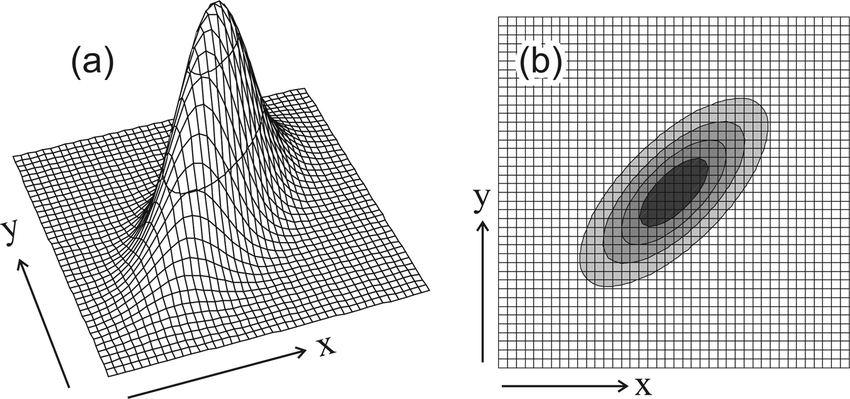
\includegraphics[width=4 in]{Images/CEF/Illustration.png}
\end{center}
\end{frame}

\begin{frame}
\begin{defn}
$\boldsymbol{X} = (X_{1}, X_{2}, \hdots, X_{N}) $ is a vector of random variables.  If $\boldsymbol{X}$ has pdf 
\begin{align*}
f(\boldsymbol{x}) & = (2 \pi)^{-N/2} \text{det}\left(\boldsymbol{\Sigma}\right)^{-1/2} \exp\left(-\frac{1}{2}(\boldsymbol{x} - \boldsymbol{\mu})^{'}\boldsymbol{\Sigma}^{-1} (\boldsymbol{x} - \boldsymbol{\mu} ) \right) 
\end{align*}
$\boldsymbol{X}$ is a \alert{Multivariate Normal} Distribution,
\begin{align*}
\boldsymbol{X} & \sim  \text{Multivariate Normal} (\boldsymbol{\mu}, \boldsymbol{\Sigma})
\end{align*}
\end{defn}
\end{frame}


\begin{frame}
$\boldsymbol{Z} = (X, Y) $ is a vector of jointly distributed random variables.
\begin{align*}
f(\boldsymbol{z}) & = (2 \pi)^{-1} \text{det}\begin{bmatrix}\sigma_x^2&\sigma_{xy}\\ \sigma_{yx}&\sigma_y^2\end{bmatrix}^{-1/2} \exp\left(-\frac{1}{2}(\begin{bmatrix}x\\y \end{bmatrix} - \begin{bmatrix}\mu_x\\\mu_y \end{bmatrix})^{'}\begin{bmatrix}\sigma_x^2&\sigma_{xy}\\ \sigma_{yx}&\sigma_y^2\end{bmatrix}^{-1}(\begin{bmatrix}x\\y \end{bmatrix} - \begin{bmatrix}\mu_x\\\mu_y \end{bmatrix} ) \right) \\
f(\boldsymbol{z}) & = \frac{1}{\sqrt{(2 \pi) (2 \pi)(\sigma_x^2\sigma_y^2-\sigma_{xy}^2)}} \exp\left(-\frac{1}{2}\begin{bmatrix}x-\mu_x\\y-\mu_y \end{bmatrix}^{'}\begin{bmatrix}\sigma_x^2&\sigma_{xy}\\ \sigma_{yx}&\sigma_y^2\end{bmatrix}^{-1}\begin{bmatrix}x-\mu_x\\y-\mu_y \end{bmatrix} \right) 
\end{align*}
\end{frame}


\begin{frame}<handout:0>
\begin{center}
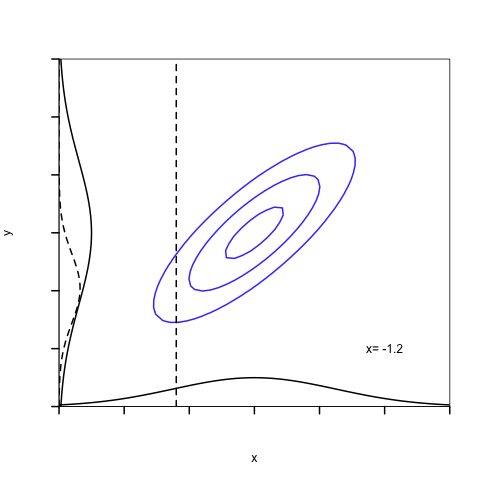
\includegraphics[width=3 in]{Images/CEF/BVN-1_2.png}
\end{center}
\end{frame}


\begin{frame}
\begin{center}
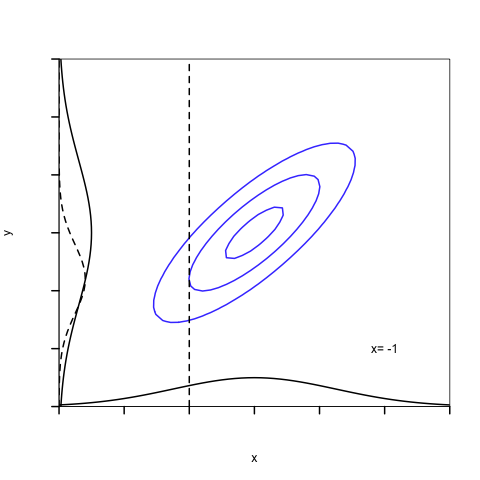
\includegraphics[width=3 in]{Images/CEF/BVN-1.png}
\end{center}
\end{frame}


\begin{frame}<handout:0>
\begin{center}
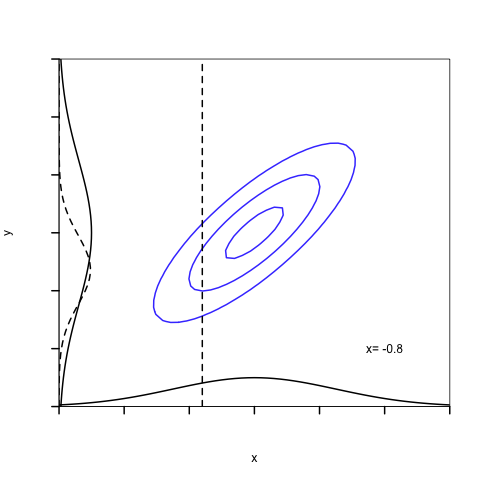
\includegraphics[width=3 in]{Images/CEF/BVN-0_8.png}
\end{center}
\end{frame}


\begin{frame}<handout:0>
\begin{center}
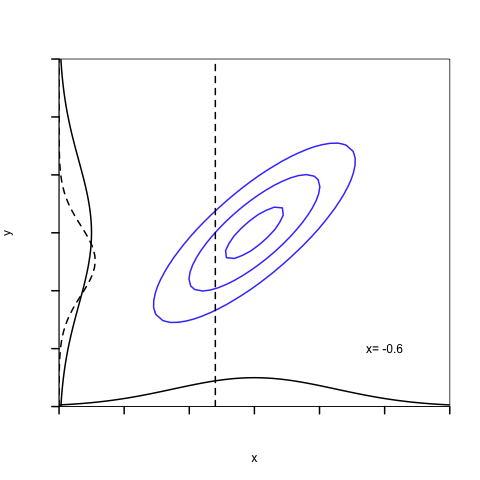
\includegraphics[width=3 in]{Images/CEF/BVN-0_6.png}
\end{center}
\end{frame}


\begin{frame}<handout:0>
\begin{center}
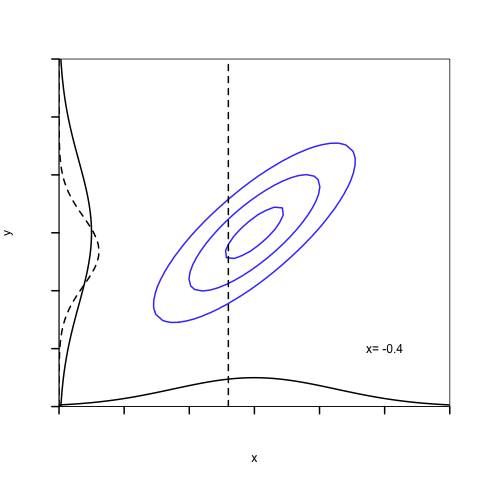
\includegraphics[width=3 in]{Images/CEF/BVN-0_4.png}
\end{center}
\end{frame}


\begin{frame}<handout:0>
\begin{center}
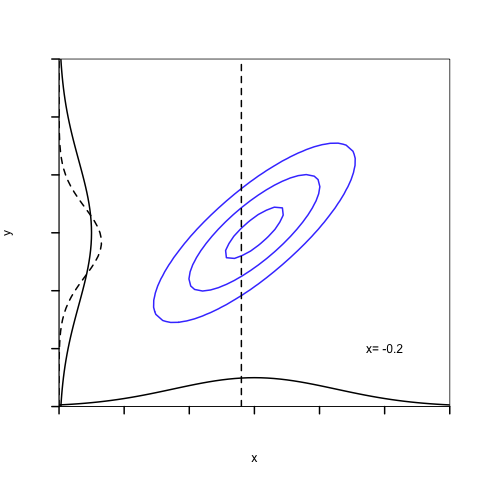
\includegraphics[width=3 in]{Images/CEF/BVN-0_2.png}
\end{center}
\end{frame}


\begin{frame}<handout:0>
\begin{center}
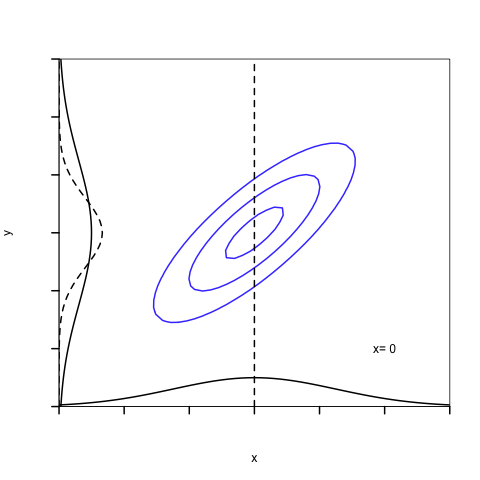
\includegraphics[width=3 in]{Images/CEF/BVN0.png}
\end{center}
\end{frame}


\begin{frame}<handout:0>
\begin{center}
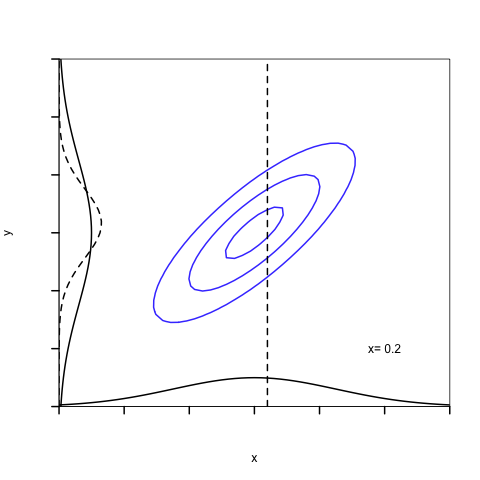
\includegraphics[width=3 in]{Images/CEF/BVN0_2.png}
\end{center}
\end{frame}


\begin{frame}<handout:0>
\begin{center}
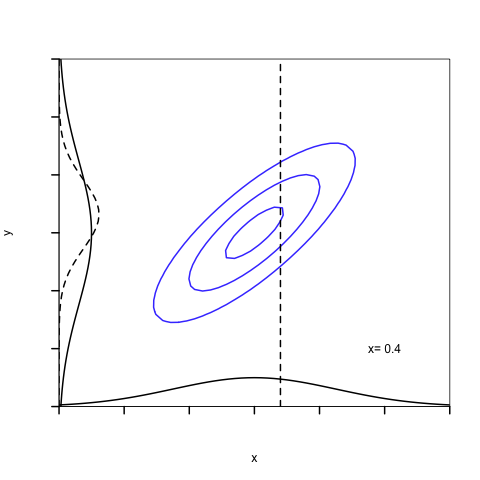
\includegraphics[width=3 in]{Images/CEF/BVN0_4.png}
\end{center}
\end{frame}


\begin{frame}<handout:0>
\begin{center}
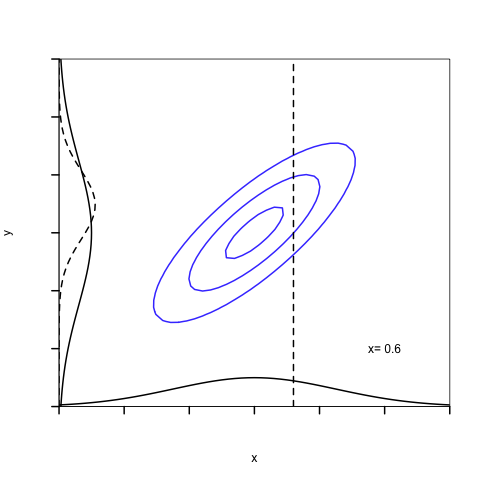
\includegraphics[width=3 in]{Images/CEF/BVN0_6.png}
\end{center}
\end{frame}


\begin{frame}<handout:0>
\begin{center}
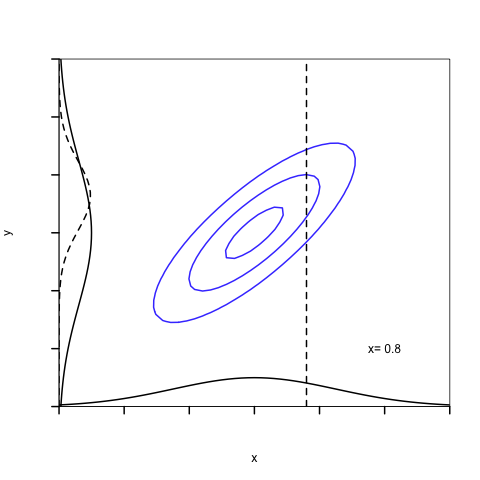
\includegraphics[width=3 in]{Images/CEF/BVN0_8.png}
\end{center}
\end{frame}


\begin{frame}<handout:0>
\begin{center}
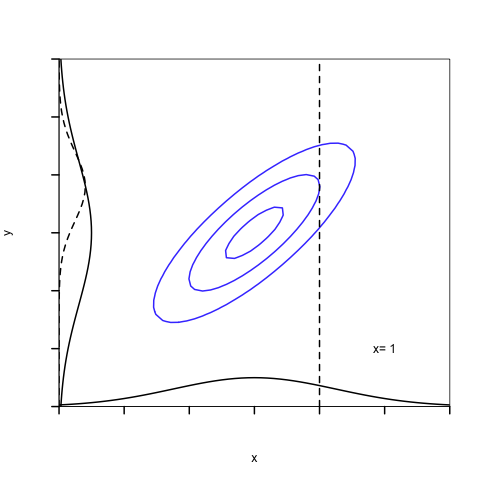
\includegraphics[width=3 in]{Images/CEF/BVN1.png}
\end{center}
\end{frame}

\begin{frame}<handout:0>
\begin{center}
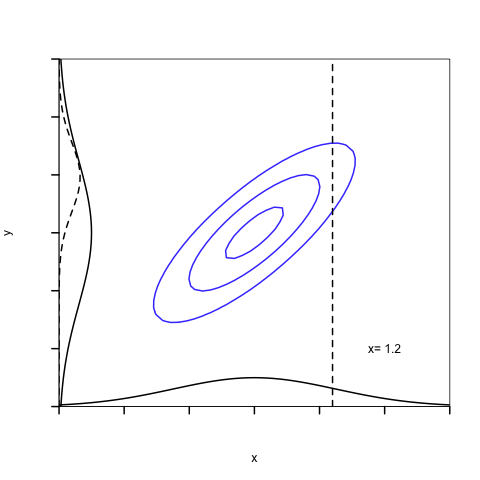
\includegraphics[width=3 in]{Images/CEF/BVN1_2.png}
\end{center}
\end{frame}


\begin{frame}
\frametitle{Prediction}
\begin{itemize}
\item If we want to predict $y$ with a known pdf.  The ``best'' prediction is $\mu_Y$ (minimum mean square error (MSE)).\pause
\item Suppose we have a bivariate distribution $f(x,y)$.  We will be told $X$.  What should we guess for $Y$?\pause
\item We can use any function $h(X)$.  What is the best, minimizing $(Y-h(X))^2$?\pause
\item We will show that only the Conditional Expectation Function $E(Y|X)$ is the best.
\end{itemize}
\end{frame}

\begin{frame}
\frametitle{Proof that CEF is the best predictor (Goldberger pg 51)}
\begin{itemize}
\item Goal: Minimize $(Y-h(X))^2$. \pause
\item Define $U\equiv Y-h(X)$, $\epsilon \equiv Y-E(Y|X)$,  $W\equiv E(Y|X)-h(X)$. \pause
\begin{align*}
U&=Y-h(X)\\\pause
U&=(\epsilon+E(Y|X))-(E(Y|X)-W)\\\pause
U&=\epsilon+W
 \end{align*}
 \pause
 \item  $W$ only depends on $X$.  So for $X=x$, let's call it $W(X=x)=w$.\pause
\begin{align*}
U^2&=\epsilon^2+2w\epsilon+w^2\\\pause
E(U^2|x)&=E(\epsilon^2|x)+2E(w\epsilon|x)+E(w^2|x)\\\pause
&=E(\epsilon^2|x)+2wE(\epsilon|x)+w^2\\\pause
&=E(\epsilon^2|x)+2w*0+w^2\\
\end{align*}
\end{itemize}
\end{frame}

\begin{frame}
\begin{align*}
E(U^2|x)&=E(\epsilon^2|x)+2w*0+w^2 &&\text{from above}\\\pause
E(U^2)&=E_X[E(U^2|X)] && \text{by Law of Iterated Expectations}\\\pause
&=E_X[E(\epsilon^2|x)+0+w^2] &&\text{Plugging in} \\ \pause
&=E[\sigma^2_{Y|x}]+E[W^2]\pause
\end{align*}
$E[W^2]\geq0$, so $E(U^2)$ is minimized if $W=0$, and recall the definition of $W$.  \pause
\begin{align*}
W&=E(Y|X)-h(X)\\\pause
0&=E(Y|X)-h(X)\\\pause
h(X)&=E(Y|X)\\
\end{align*}
The Conditional Expectation Function $E(Y|X)$ *is* the function that minimizes $E(U^2)$.
\end{frame}



\begin{frame}
\frametitle{Conditional Expectation as a Prediction}
Suppose $Y$ and $X$ are random variables.

\begin{align*}
\mu_{Y|X}& \equiv  E[Y|X] 
\end{align*}\pause
$\mu_{Y|X}$ is our best guess for $Y$ given $X$\\\pause
$\epsilon$ is the amount we are off.
\begin{align*}
\epsilon & \equiv Y-\mu_{Y|X}
\end{align*}


\end{frame}


\begin{frame}
\frametitle{Properties of Estimation error}
$\epsilon$ is a random variable where:
\begin{align*}
E[\epsilon|X] & =  E[Y- \mu_{Y|X}|X] \\\pause
 & =  E[Y|X]-E[ \mu_{Y|X}|X] \\\pause
  & =   E[Y|X]-E[ E[Y|X]|X]\\\pause
  & =  \mu_{Y|X} -\mu_{Y|X} =0 
\end{align*}\pause
By the law of iterated expectations:\pause
\begin{align*}
E[\epsilon] & =  E[E[ \epsilon|X]]=0
\end{align*}\pause
The disturbances center on 0 \emph{by construction}.  

\end{frame}


\begin{frame}
\frametitle{Covariance of  Estimator and Disturbance}
\begin{align*}
E[\epsilon \mu_{Y|X}] & =  E[E[\epsilon \mu_{Y|X}|X]]=E[\mu_{Y|X}E[\epsilon|X]]=E[\mu_{Y|X}*0]=0 
\end{align*}\pause
because $\mu_{Y|X}$ only depends on $X$.\pause
\begin{align*}
Cov(\epsilon , \mu_{Y|X}) & =  E[ \epsilon \mu_{Y|X}]-E[\epsilon ]E[\mu_{Y|X}]=0- 0*\mu_{Y|X}=0
\end{align*}\pause
The disturbance is uncorrelated with the conditional expectation.  This is what allows us to separate the signal from the noise.
\end{frame}


\begin{frame}
\frametitle{Discussion of CEF}
\begin{itemize}
\item CEF solves the minimum mean squared error (MSE) prediction problem.
\item But it depends on knowing the conditional distribution of $Y|x$, because $E[Y|X]=\int y f_{Y|x}(y|x)dy$.\pause
\item This is a general problem: MSE minimizing estimators often require knowledge about the population.\pause
\item Instead we will restrict attention to linear predictors. \pause  We seek to find the "best" linear predictor (BLP). \pause
\item Later we will show that OLS regression estimates are BLUE (best linear unbiased estimators) \textbf{if} the CEF is linear and residuals are constant. \pause
\item However, what if the CEF is not linear? \pause
\item Linear regression is the best (minimum MSE) linear approximation to the CEF. 
\end{itemize}
\end{frame}

\section{Linear Predictors}

\begin{frame}{(Best) Linear Predictors}

\begin{itemize}
\item Suppose we want a predictor $E(Y|X)$ that is \textbf{linear}:
$$f(X)=a+bX$$\pause
Our standard for prediction is to minimize the mean-square error (best): \\
\item Whereas the CEF might be infinitely complex, the BLP is characterized just by two numbers, $a$ and $b$.\pause \ If the CEF is linear, the BLP is the CEF.\\
\pause
Choose $a$ and $b$ to minimize
$$M=E[(Y-(a+bX))^2]$$
\end{itemize}
\end{frame}

\begin{frame}
\frametitle{Best Linear Predictor (a)}
Take partial derivative with respect to $a$.\pause
\begin{align*}
\frac{\partial E[(Y-(a+bX))^2]}{\partial a} &= E[\frac{\partial(Y-(a+bX))^2}{\partial a}]\\\pause
&= E[ -2(Y-(a+bX))]
\end{align*} \pause
setting equal to 0:\pause
\begin{align*}
0&=  E[-2(Y)-(a+bX)]\\\pause
0&=  -2E[Y]+2E(a+bX)\\\pause
E(Y)&= a+bE(X)\\\pause
E(Y)-bE(X)&= a
\end{align*} 
\end{frame}

\begin{frame}
\frametitle{Best Linear Predictor (b)}
Take partial derivative with respect to $b$.\pause
\begin{align*}
\frac{\partial E[(Y-(a+bX))^2]}{\partial b}&= E[\partial(Y-(a+bX))^2/\partial b]\\\pause
&= 2E[(Y-(a+bX))(-X)]\pause
\end{align*} 
setting equal to 0:\pause
\begin{align*}
0&= -2E[(YX)-(a+bX)(X)]\\\pause
0&= -2E(YX)+2E[(a+bX)(X)]
\end{align*} 
\end{frame}


\begin{frame}{Best Linear Predictor (b continued)}
\begin{align*}
0&= -2E[YX]+2E[(a+bX)(X)]\\\pause
E(YX)&= aE(X)+bE(X^2)\\\pause
E(YX)&= [E(Y)-bE(X)]E(X)+bE(X^2)\\\pause
E(YX)&= E(Y)E(X)-bE(X)E(X)+bE(X^2)\\\pause
E(YX)-E(Y)E(X)&= b[E(X^2)-E(X)^2]\\\pause
b&=\frac{E(YX)-E(Y)E(X)}{[E(X^2)-E(X)^2]}=\frac{Cov(X,Y)}{Var(X)}\\
\end{align*} 
\end{frame}

\begin{frame}{Best Linear Predictor}
\begin{align*}
E[Y|X]&=\beta_0+\beta_1X\\\pause
Y&=\beta_0+\beta_1X+\epsilon
\end{align*} 
\begin{itemize}\pause
\item Parameters (in Greek)
\begin{itemize}
\item $\epsilon=Y-E[Y|X]$
\item The slope $\beta =\frac{Cov(X,Y)}{Var(X)}$
\item The intercept $\alpha=E(Y)-\beta E(X)$
\end{itemize}\pause
\item $Y$ is called the dependent variable, $X$ is called the independent variable.
\end{itemize}
\end{frame}

\begin{frame}{What is "linear in parameters"?}
\begin{itemize}
\item The Best Linear Predictor is linear in \emph{parameters} $\theta\in\{\beta_0,\ \beta_1\ \ldots\}$.\pause
\item Examples of linear in parameters: 
\begin{align*}
Y&=\beta_0+\beta_1X^{4}+\epsilon\\
Y&=\beta_0+\beta_1e^{X}+\epsilon
\end{align*}  \pause
\item Examples of nonlinear in parameters:
\begin{align*}
Y&=\beta_0+\frac{1}{\beta_1}X+\epsilon\\
Y&=\beta_0+\beta_1^2 X+\epsilon\\
Y&=\beta_0+e^{\beta_1 X}+\epsilon
\end{align*} 
\end{itemize}

\end{frame}



\begin{frame}
\frametitle{Deriving variance of BLP at minimized values}
\begin{align*}
\beta &=\frac{Cov(X,Y)}{Var(X)}&&  \beta Var(X)=Cov(X,Y)
\end{align*}  \pause
\begin{align*}
E[(Y-(\alpha+\beta X))^2]-E[Y-(\alpha+\beta X)]^2 &=Var(Y-(\alpha+\beta X))\\\pause
&=Var(Y-\beta X)\\\pause
&=Var(Y)+Var(\beta X)-2 Cov(\beta X,Y)\\\pause
 &=Var(Y)+\beta^2Var(X)-2\beta Cov(X,Y)\\\pause
 &=Var(Y)+\beta^2Var(X)-2\beta^2 Var(X)\\\pause
  &=Var(Y)-\beta^2 Var(X)\\\pause
  \sigma^2_\epsilon  &=\sigma^2_Y-\beta^2 \sigma^2_X\\
\end{align*} 
\end{frame}



\begin{frame}
\frametitle{Example Best Linear Predictor, roof}
Example: $X + Y$\\
Suppose $X$ and $Y$ have pdf $x + y$ for $x, y \in [0,1]$.  \pause \\
\pause
$$b=\frac{Cov(X,Y)}{Var(X)} = -1/11$$
$$a=E(Y)-bE(X)= 84/132$$
\end{frame}


\begin{frame}
\begin{center}
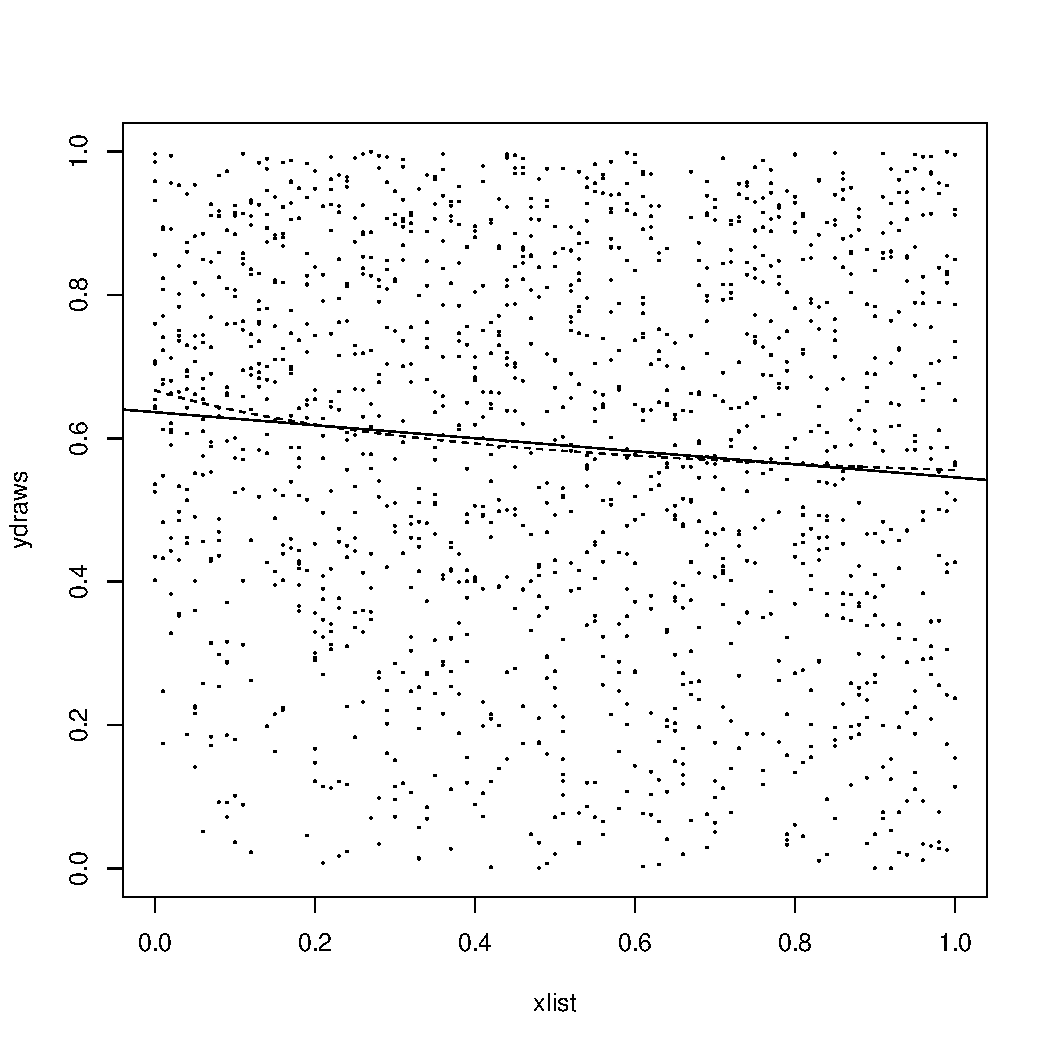
\includegraphics[width=3 in]{Images/ConditionalExp.pdf}
\end{center}
\end{frame}

\begin{frame}
\begin{center}
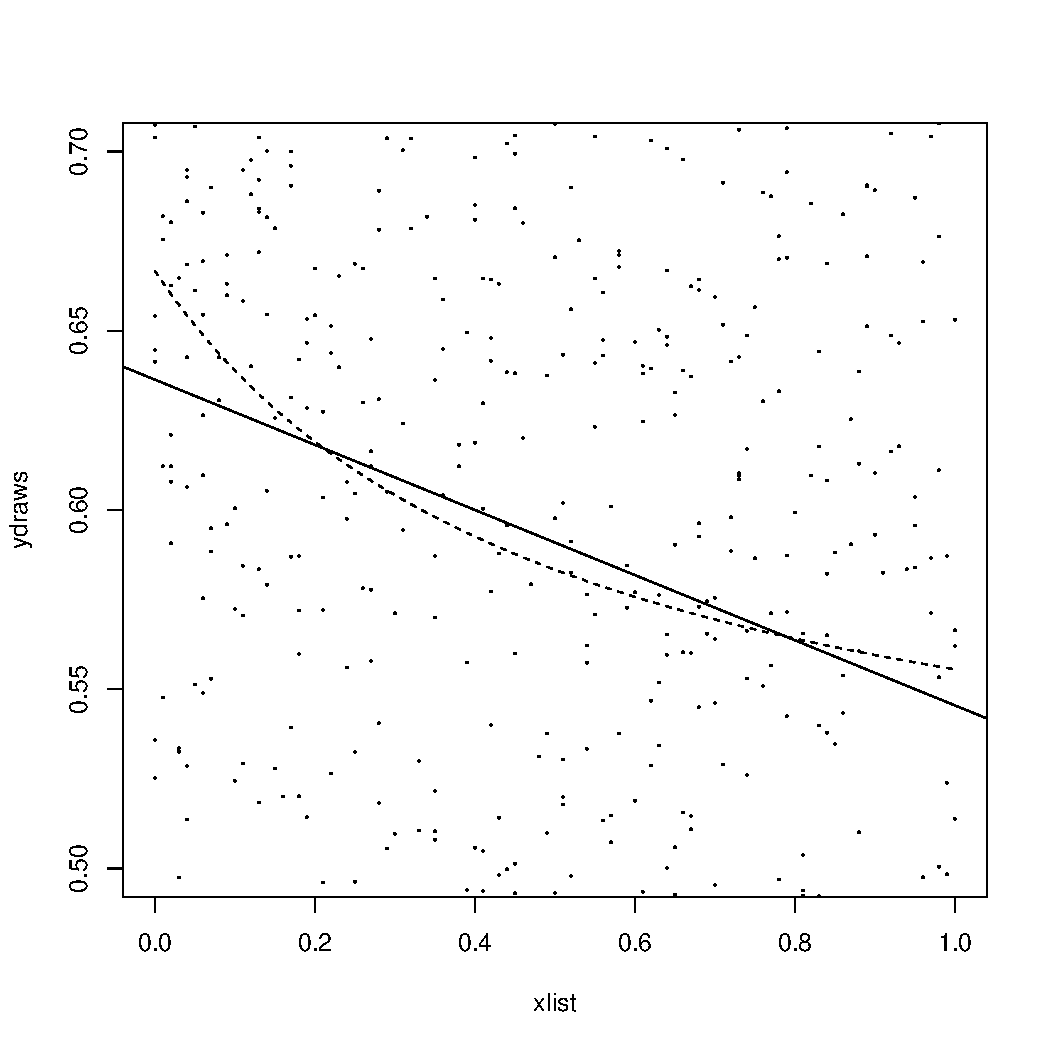
\includegraphics[width=3 in]{Images/ConditionalExpZoom.pdf}
\end{center}
\end{frame}

\begin{frame}<handout:0>
\begin{center}

\includegraphics[width=2.5 in]{Images/platoaristotle.jpeg}
\end{center}
\end{frame}

\begin{frame}{Sample vs Population}
\begin{itemize}
\item Theoretical "Population" Objects (not observed): Greek Letters: $\alpha$, $\beta$, $\mu$, $\sigma$, $\epsilon$,  \ E(), Var(), Cov().
\item Empirical Objects (observed): latin letters, $a$, $b$, $\bar{x}$, $s^2$, $e$, $\widehat{E}()$, $\widehat{Cov}()$.
\item Objects of the first group are not exactly equal to their empirical analogues from the second group.
\begin{itemize}
\item $\alpha=\mu_Y-\beta\mu_X$ is correct.
\item $a=\bar{y}-b\bar{x}$ is correct.
\item $E(\bar{x})=\mu$ is correct.
\item $\bar{x}=\mu$ is not correct. 
\item $Cov(x)=s^2_x$ is not correct.
\end{itemize}
\end{itemize}
\end{frame}

\section{Estimating BLP with OLS}
\begin{frame}
\frametitle{Sample Linear projection}
Population linear projection:
$$E(Y|X)=\alpha+\beta X\pause$$
where $$\beta=\frac{\sigma_{XY}}{\sigma^2_X},\ \  \alpha=\mu_Y-\beta\mu_X$$\pause
\\
\emph{Sample} linear projection:
$$\hat{Y}=b_0+b_1X$$
where $$b_1=\frac{S_{XY}}{S^2_X},\ b_0=\bar{Y}-b_1\bar{X}$$

\end{frame}

\begin{frame}
\frametitle{Asymptotic Distribution of Sample Slope}
Call $X^*=X-\bar{X}$, $\epsilon=Y-(\alpha+\beta X)$, then the Bivariate Delta Method (Goldberg 10.5) tells us
$$b_1\stackrel{A}{\sim }N(\beta, \frac{E(X^{*2}\epsilon^2)}{(\sigma^2_X)^2})$$\pause
If $E(\epsilon^2|X)$ is a constant $\sigma^2$, then
\begin{align*}
E(X^{*2}\epsilon^2)&=E_X[E(X^{*2}\epsilon^2|X)]=E_X[X^{*2}E(\epsilon^2|X)]\\\pause
&=E_X[X^{*2}\sigma^2]\\\pause
&=\sigma^2E_X[X^{*2}]=\sigma^2V(X)=\sigma^2\sigma^2_X\pause
\end{align*} 
$$b_1\stackrel{A}{\sim }N(\beta, \frac{\sigma^2}{\sigma^2_X})$$
\end{frame}


\begin{frame}{Ordinary Least Squares Regression Estimator}
\begin{itemize}
\item In our effort to approximate the CEF, we simply replaced the expectations, covariances etc. in the BLP with the sample means, covariances etc.\pause
\item It turns out that we can algebraically process data with the least squares procedure (OLS) to estimate the BLP parameters.\pause
\item That is, we will solve $\min_{b_0,\ b_1} \sum_i e^2$\pause
\item In addition, \textbf{if} the CEF function is linear and $E(\epsilon^2|X)$ is a constant $\sigma^2$, then the Gauss Markov Theorem tells us that OLS is a Best Linear Unbiased Estimator (BLUE).
\end{itemize}
\end{frame}


\begin{frame}{Brief Linear Algebra Interlude}
\begin{itemize}
\item $\bm{x}=\begin{bmatrix} x_1 \\ x_2 \\ \ldots \\ x_n \end{bmatrix}$ is $n \times 1$ column vector.  $\bm{i}=\begin{bmatrix}   1\\ 1\\ \ldots\\ 1\end{bmatrix}$.  \pause
\item $\bm{x'}=\bm{x^{T}}=\begin{bmatrix} x_1 & x_2 & \ldots & x_n \end{bmatrix}$ is $1 \times n$ vector.\pause
\item If $c$ is a scalar, $c\bm{x'}=\begin{bmatrix} cx_1 & cx_2 & \ldots & cx_n \end{bmatrix}$.
\item $\bm{x'i}=\bm{x\cdot i}= x_1*1+x_2*1+x_3*1+ \ldots+ x_n*1=\sum x_i=n\bar{x}$\pause
\item $\bm{x'x}= x_1^2+x_2^2+x_3^2+ \ldots+ x_n^2=\sum x_i^2=n*\widehat{Var}(x)+n\bar{x}^2$\pause
\item $\bm{xx'}=\begin{bmatrix} x_1x_1& x_1x_2&\ldots\\  x_2x_1&\ldots\\ \ldots \end{bmatrix}$, \quad $\bm{I}=\begin{bmatrix} 1& 0&\ldots\\ 0&1&\ldots\\ \ldots  \end{bmatrix}$
\end{itemize}
\end{frame}


\begin{frame}{Linear Algebra Rules}
If $\bm{x}$, $\bm{y}$, and $\bm{z}$ are vectors of equal length: 
\begin{itemize}
\item You can add, subtract and dot product them.  No division of vectors. 
\item Commutative property: If $\bm{x}$ and $\bm{y}$ are vectors of equal length, $\bm{x'y}=\bm{y'x}$
\item Distributive property: $\bm{x'(y+z)}=\bm{x'y}+\bm{x'z}$
\end{itemize}
\end{frame}

\begin{frame}{Linear Algebra Geometry (Advanced Topic)}
\begin{itemize}
\item $\sqrt{\bm{x}'\bm{x}}=||\bm{x}||$ is called the Euclidean Norm, from the classic Euclidean distance $\sqrt{a^2+b^2}=c$ in Descartes' theory of coordinates.
\item $\bm{u}=\frac{\bm{x}}{\sqrt{\bm{x}'\bm{x}}}$ is called the \textbf{unit vector} in the direction of $\bm{x}$.
\item If $\bm{u}$ is a unit vector in the direction of $\bm{x}$, $\bm{y'u}=\bm{u'y}$ is the *scalar projection* of $\bm{y}$ onto $\bm{x}$.
\item $\bm{(u'y) u}$ is the *vector projection* of $\bm{y}$ onto $\bm{x}$. 
$$\bm{(u'y) u}=\left(\frac{\bm{x'}\bm{y}}{\sqrt{\bm{x}'\bm{x}}}\right) \frac{\bm{x}}{\sqrt{\bm{x}'\bm{x}}}=\left(\frac{\bm{x'}\bm{y}}{\bm{x}'\bm{x}}\right) \bm{x}$$
\item If $\bm{x'y}=0$, $\bm{x}$ is "orthogonal" to $\bm{y}$.
\end{itemize}
\end{frame}


\begin{frame}{Gauss-Markov Assumptions (classical fixed $\bm{x}$)}
\begin{enumerate}
\item CEF is linear\pause
\item $\bm{x}=\begin{bmatrix} x_1\\ x_2\\ \ldots\\ x_n\end{bmatrix}$ is fixed.\pause
\item $\sum_{i=1}^n (x_i - \bar{x})^2>0$ [x takes on at least two values]. \pause
\item $E(\epsilon_i)=0\ \ \forall i$.\pause
\item $E(\bm{\epsilon}\bm{\epsilon}^{'})=\sigma_\epsilon^2\bm{I}$.\pause
\begin{itemize}
\item $Var(\epsilon_i)=\sigma_\epsilon^2\ \ \forall i$ [homoskedasticity, i.i.d.]\pause
\item $Cov(\epsilon_i,\epsilon_j)=0$
\end{itemize}
\end{enumerate}
\end{frame}


\begin{frame}{Deriving $b_0,\ b_1$ estimator using OLS}
 \begin{align*}
  &\min_{b_0\ b_1} \sum_i e^2=\min_{b_0\ b_1} \bm{e'}\bm{e}\pause
\end{align*} 
  \begin{columns}
  \begin{column}{.4\textwidth}
 \begin{align*}
  \frac{\partial}{\partial b_1}\bm{e'}\bm{e}&= \frac{\partial}{\partial b_1} (\bm{y}-\bm{\hat{y}})^{'} (\bm{y}-\bm{\hat{y}})\\\pause
&= \frac{\partial}{\partial b_1} (\bm{y}^{'}\bm{y}-\bm{y^{'}}\bm{\hat{y}}- \bm{\hat{y}^{'}}\bm{y}+\bm{\hat{y}^{'}}\bm{\hat{y}})\\\pause
&= \frac{\partial}{\partial b_1} (\bm{y}^{'}\bm{y}-2\bm{\hat{y}^{'}}\bm{y}+\bm{\hat{y}^{'}}\bm{\hat{y}})\\\pause
&= 0-2\frac{\partial}{\partial b_1}\bm{\hat{y}^{'}y}+\frac{\partial}{\partial b_1}\bm{\hat{y}^{'}}\bm{\hat{y}}\pause
\end{align*}
\end{column}
  \begin{column}{.4\textwidth}
 \begin{align*}
  \frac{\partial}{\partial b_0}\bm{e'}\bm{e}&= \frac{\partial}{\partial b_0} (\bm{y}-\bm{\hat{y}})^{'} (\bm{y}-\bm{\hat{y}})\\\pause
 &= 0-2\frac{\partial}{\partial b_0}\bm{\hat{y}^{'}y}+\frac{\partial}{\partial b_0}\bm{\hat{y}^{'}}\bm{\hat{y}}
\end{align*}
  \end{column}
  \end{columns}
\end{frame}

\begin{frame}{Note on calculus with vectors (I)}
$$\bm{\hat{y}}=\begin{bmatrix} b_0+b_1 x_1 \\  b_0+b_1 x_2 \\   b_0+b_1 x_3 \\ \ldots \end{bmatrix}\ \quad \quad \frac{\partial\bm{\hat{y} }}{\partial b_1}=\begin{bmatrix} x_1  \\ x_2 \\ x_3 \\ \ldots \end{bmatrix}=\bm{x}\ \quad \quad \frac{\partial\bm{\hat{y} }}{\partial b_0}=\begin{bmatrix} 1 \\ 1 \\ 1 \\ \ldots \end{bmatrix}=\bm{i}$$\pause
  $$\bm{\hat{y}^{'}}\bm{\hat{y}}=\begin{bmatrix}  b_0+b_1 x_1&  b_0+b_1 x_2 &  b_0+b_1 x_3 & \ldots \end{bmatrix}\begin{bmatrix} b_0+b_1 x_1 \\  b_0+b_1x_2 \\  b_0+b_1 x_3 \\ \ldots \end{bmatrix}= \sum_i (b_0+b_1x_i)^2$$
\end{frame}


\begin{frame}{Note on calculus with vectors (II)}

\begin{align*}
\frac{\partial}{\partial b_1}\bm{\hat{y}^{'}}\bm{\hat{y}}&=\frac{\partial}{\partial b_1} \sum_i (b_0+b_1x_i)^2 \\
&=\sum_i 2 x_i (b_0+b_1x_i)\\ 
&=2\bm{x'} [b_0\bm{i}+b_1\bm{x}]\\\pause
\frac{\partial}{\partial b_0}\bm{\hat{y}^{'}}\bm{\hat{y}}&= \sum_i 2(b_0+b_1x_i)\\
&=2  \bm{i^{'}}[b_0+b_1\bm{x}]
\end{align*}
\end{frame}

\begin{frame}{Deriving $b_0,\ b_1$ estimator using OLS}
  \begin{columns}
  \begin{column}{.4\textwidth}
\begin{align*}
   \frac{\partial}{\partial b_0}\bm{e'}\bm{e}&=  0-2\frac{\partial}{\partial b_0}\bm{\hat{y}^{'}y}+\frac{\partial}{\partial b_0}\bm{\hat{y}^{'}}\bm{\hat{y}}\\\pause
  &= 0-2\bm{i^{'}}\bm{y}+2 \bm{i^{'}}[(b_0+b_1\bm{x})]\\\pause
  \bm{i^{'}}b_0 &=\bm{i^{'}}\bm{y}-b_1\bm{i^{'}}\bm{x}\\\pause
   nb_0 &=\bm{i^{'}}\bm{y}-b_1\bm{i^{'}}\bm{x}\\\pause
    nb_0 &= n\bar{y}-b_1n\bar{x}\\\pause
      b_0 &= \bar{y}-b_1\bar{x}\pause
    \end{align*}
\end{column}
  \begin{column}{.5\textwidth}
\begin{align*}
     \frac{\partial}{\partial b_1}\bm{e'}\bm{e}&= 0-2\frac{\partial}{\partial b_1}\bm{\hat{y}^{'}y}+\frac{\partial}{\partial b_1}\bm{\hat{y}^{'}}\bm{\hat{y}}\\\pause
  &= -2\bm{x'y}+2\bm{x'}[b_0\bm{i}+b_1\bm{x}]\\\pause
&= -2\bm{x'y}+2\bm{x'}[[\bar{y}-b_1\bar{x}]\bm{i}+b_1\bm{x}]\\\pause
&= -2\bm{x'y}+2\bm{x'}\bar{y}\bm{i}+2\bm{x' }b_1(\bm{x}-\bar{x}\bm{i})\\\pause
&= -2\bm{x'y}+2n\bar{x}\bar{y}+2b_1[\bm{x' x}-n\bar{x}\bar{x}]\\\pause
\bm{x'y}-n\bar{x}\bar{y}&=b_1[\bm{x' x}-n\bar{x}\bar{x}]\\\pause
\widehat{Cov}(\bm{x,\ y})&=b_1\widehat{Var}(\bm{x})\\\pause
\frac{\widehat{Cov}(\bm{x},\bm{y})}{\widehat{Var}(\bm{x})}&=b_1 \quad \text{By assumption 3}
\end{align*}
 \end{column}
 \end{columns}
\end{frame}



\begin{frame}[fragile]
  \begin{lstlisting}
>  x <- 1:50
>  y <- 8 + .5 * x + rnorm(50)

>  coef(lm(y~x))
(Intercept)     x 
8.1679311   0.4982869 

>  mean(y) - cov(x,y) / var(x) * mean(x)
[1] 8.167931
>  cov(x,y)/var(x)
[1] 0.4982869
   \end{lstlisting}
\end{frame}





\section{OLS properties}

\begin{frame}{Interpretation}
\begin{itemize}
\item $b_1$ is the slope: one unit change in $x$ is associated with a $b_1$ unit change in $Y$.\pause
\begin{eqnarray*}
\bm{\hat{y}}=b_0+\frac{\widehat{Cov}(\bm{x},\bm{y})}{\widehat{Var}(\bm{x})}\bm{x}\\
\bm{y}=\bm{\hat{y}}+\bm{e}
\end{eqnarray*}\pause
\item $b_0$ is the intercept: What is the predicted value of y when $x=0$.\pause
\item $e_i$ is the residual: observed y minus predicted y.
\end{itemize}
\end{frame}

\begin{frame}{Decomposition of Variance}
\begin{align*}
\sigma^2_\epsilon &= \sigma^2_Y-\beta^2 \sigma^2_X\\\pause
\widehat{Var}(\bm{e}) &= \widehat{Var}(\bm{y})-b_1^2 \widehat{Var}(\bm{x})\\\pause
b_1^2 \widehat{Var}(\bm{x})+\widehat{Var}(\bm{e})&= \widehat{Var}(\bm{y})\\\pause
\underset{\text{Explained Sum of Squares}}{b_1^2 \sum (x_i-\bar{x})^2}+\underset{\text{Residual Sum of Squares}}{\sum e_i^2}&=\underset{\text{Total Sum of Squares}}{\sum(y_i-\bar{y})^2}\\\pause
\text{ESS}+\text{RSS}&=\text{TSS}\\\pause
\frac{\text{ESS}}{\text{TSS}}+\frac{\text{RSS}}{\text{TSS}}&=1\\\pause
R^2+\frac{\text{RSS}}{\text{TSS}}&=1
\end{align*}
\end{frame}

\begin{frame}
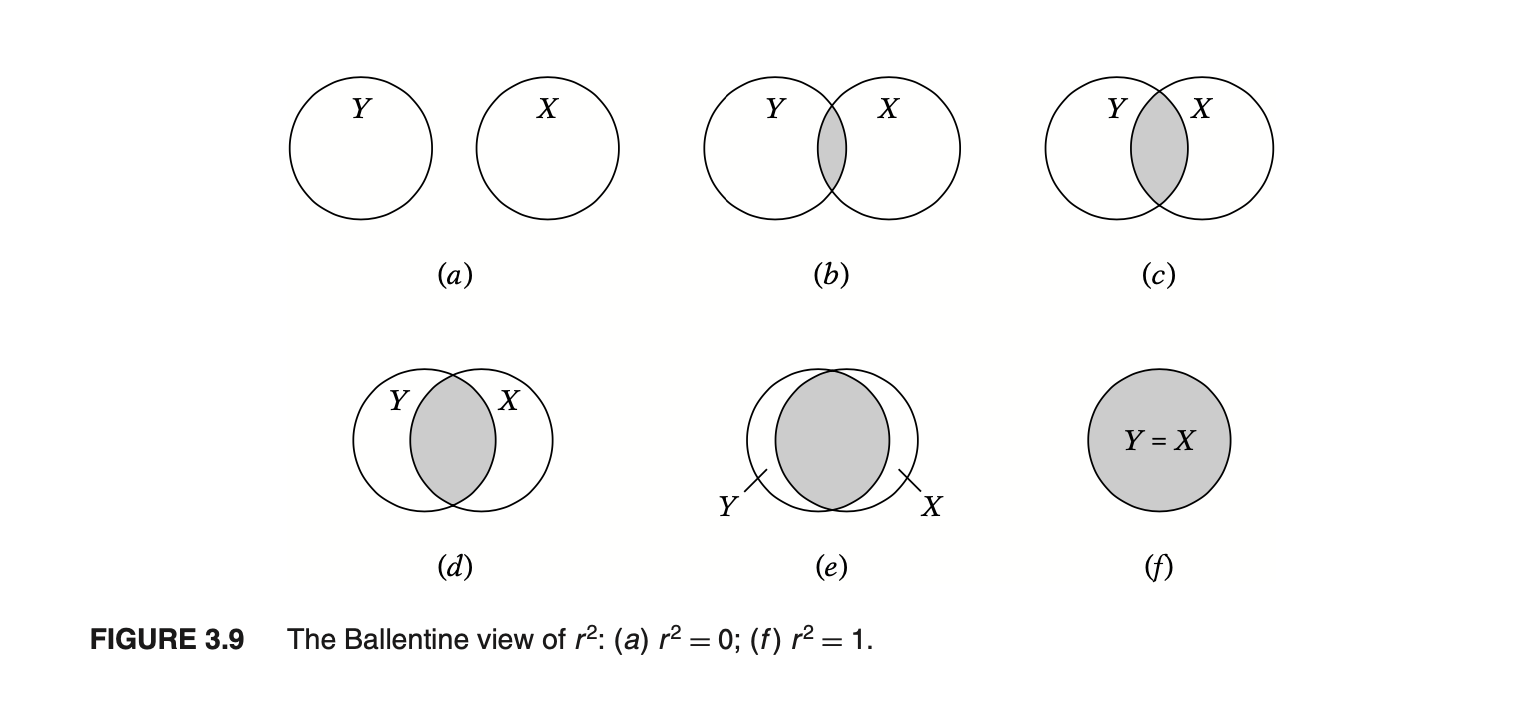
\includegraphics[width=5 in]{Images/Ballentine.png}
\end{frame}


\begin{frame}{Sample Correlation Coefficient}
$$r_{xy}\equiv \frac{\widehat{Cov}(\bm{x},\ \bm{y})}{\sqrt{\widehat{Var}(\bm{x})}\sqrt{\widehat{Var}(\bm{y})}}=\frac{S_{XY}}{S_XS_Y}=\frac{\frac{1}{n-1}\sum(x_i-\bar{x})(y_i-\bar{y})}{\sqrt{\frac{1}{n-1}\sum(x-\bar{x})^2\frac{1}{n-1}\sum(y_i-\bar{y})^2}}$$
\begin{itemize}
\item The correlation coefficient ($r_{xy}$)is the normalized linear relationship.
\item The OLS slope coefficient ($b_1$) is the unnormalized linear relationship. 
\end{itemize}
\end{frame}

\begin{frame}{OLS coefficient vs Correlation}
\begin{align*}
b_1&=\frac{\widehat{Cov}(\bm{x},\ \bm{y})}{\sqrt{\widehat{Var}(\bm{x})}} \frac{1}{\sqrt{\widehat{Var}(\bm{x})}} \tag{Definition of $b_1$}\\\pause
\frac{b_1}{\sqrt{\widehat{Var}(\bm{y})}}&=\frac{\widehat{Cov}(\bm{x},\ \bm{y})}{\sqrt{\widehat{Var}(\bm{x})}\sqrt{\widehat{Var}(\bm{y})}} \frac{1}{\sqrt{\widehat{Var}(\bm{x})}}\\\pause
&=r_{xy} \frac{1}{\sqrt{\widehat{Var}(\bm{x})}} \\\pause
b_1&=r_{xy} \frac{\sqrt{\widehat{Var}(\bm{y})}}{\sqrt{\widehat{Var}(\bm{x})}}=r_{xy}\frac{S_Y}{S_X}
\end{align*}
\end{frame}



\begin{frame}[fragile]
  \begin{lstlisting}
>  x <- 1:50
>  y <- 8 + .5 * x + rnorm(50)

>  coef(lm(y~x))
(Intercept)     x 
8.1679311   0.4982869 

> cor(x,y)
[1] 0.9897854

> cor(x,y)*sd(y)/sd(x)
[1] 0.4982869

   \end{lstlisting}
\end{frame}



\begin{frame}{Obtaining the Sample Correlation Coefficient from a Regression}
\begin{align*}
\bm{\hat{y}}&=b_0+b_1\bm{x}\\\pause
\bm{\hat{y}}&= \bar{y}-b_1\bar{x}+b_1\bm{x}\\\pause
\bm{\hat{y}}-\bar{y}&=b_1(\bm{x}-\bar{x})\\\pause
\bm{\hat{y}}-\bar{y}&=r_{xy}\frac{S_Y}{S_X}(\bm{x}-\bar{x})\\\pause
\frac{\bm{\hat{y}}-\bar{y}}{S_Y}&=r_{xy}\frac{(\bm{x}-\bar{x})}{S_X}\\ \pause
y^*&=\rho_0+\rho_1 x^*
\end{align*}
\end{frame}


\begin{frame}[fragile]
  \begin{lstlisting}
> x <- 1:50
> y <- 8+ .5 * x + rnorm(50,sd=3)
> 
> cor(x,y)
[1] 0.9139259
> 
> yhatnorm <- (predict(lm(y~x))-mean(y))/sd(y)
> xhatnorm <- (x-mean(x))/sd(x)
> 
> coef(lm(yhatnorm ~ xhatnorm -1 ))
 xhatnorm 
0.9139259 
   \end{lstlisting}
\end{frame}


\begin{frame}{Proof that OLS unbiased Bias($\hat{\theta})\equiv E(\hat{\theta})-\theta$}
\begin{itemize}
\item Assume specification : $\bm{y}=[\beta_0\bm{i}+\beta_1\bm{x}+\bm{\epsilon}]$,\quad $\bm{i'}\bm{y}=[\bm{i'}\beta_0\bm{i}+\bm{i'}\beta_1\bm{x}+\bm{i'}\bm{\epsilon}]$,\quad  $\bar{y}=\beta_0+\beta_1\bar{x}+\bar{\epsilon}$\pause
\begin{align*}
b_1&=\frac{\bm{x'y}-n\bar{x}\bar{y}}{\widehat{Var}(x)}\\\pause
b_1&=\frac{\bm{x'}[\beta_0\bm{i}+\beta_1\bm{x}+\bm{\epsilon}]-n\bar{x}[\beta_0+\beta_1\bar{x}+\bar{\epsilon}]}{\widehat{Var}(x)}\\\pause
&=\frac{n\bar{x}\beta_0-n\bar{x}\beta_0+\bm{x'}\beta_1\bm{x}-n\bar{x}\beta_1+\bm{x'}\bm{\epsilon}-n\bar{x}\bar{\epsilon}}{\widehat{Var}(x)}\\\pause
&=\frac{\beta_1[\bm{x'}\bm{x}-n\bar{x}]+\bm{x'}\bm{\epsilon}-n\bar{x}\bar{\epsilon}}{\widehat{Var}(x)}\\\pause
&=\beta_1+\frac{\bm{x'}\bm{\epsilon}-n\bar{x}\bar{\epsilon}}{\widehat{Var}(x)}
\end{align*}
\end{itemize}
\end{frame}


\begin{frame}{Proof that OLS unbiased}
\begin{itemize}
\item Bias($\hat{\theta})\equiv E(\hat{\theta})-\theta$\pause
\begin{align*}
b_1&=\beta_1+\frac{\bm{x'}\bm{\epsilon}-n\bar{x}\bar{\epsilon}}{\widehat{Var}(x)}\\\pause
E[b_1]&=E[\beta_1]+E[\frac{\bm{x'}\bm{\epsilon}-n\bar{x}\bar{\epsilon}}{\widehat{Var}(x)}]\\\pause
E[b_1]&=E[\beta_1]+\frac{ \bm{ x' }E[\bm{\epsilon}]-n\bar{x}E[ \bar{ \epsilon }] }{ \widehat{Var}(x) } \quad \text{by assumption (2)}\\\pause
E[b_1]&=E[\beta_1]+\frac{\bm{x'}0-n\bar{x}0}{\widehat{Var}(x)}
\end{align*}
\end{itemize}
\end{frame}




\begin{frame}{Change of Notation}
\begin{itemize}
\item The notation simplifies if we center our variables $\bm{\tilde{x}}=\bm{x}-\bar{x}$, $\bm{\tilde{y}}=\bm{y}-\bar{y}$, \pause
\item $b_1= \frac{\bm{\tilde{x}'\tilde{y}}}{\bm{\tilde{x}'\tilde{x}}}$\pause
\item Note: $b_1\bm{\tilde{x}}=\frac{\bm{\tilde{x}'\tilde{y}}}{\bm{\tilde{x}'\tilde{x}}}\bm{\tilde{x}}$ is the vector projection of $\bm{y}$ in $\bm{\tilde{x}}$.
\item Define weights $\bm{w}\equiv \frac{\bm{\tilde{x}}}{\bm{\tilde{x}'\tilde{x}}}$\pause
\item Note $\bm{w'}\bm{w}= \frac{\bm{\tilde{x}'\tilde{x}}}{\bm{(\tilde{x}'\tilde{x})'\tilde{x}'\tilde{x}}}=\frac{1}{\bm{(\tilde{x}'\tilde{x})'}}$\pause
\item $b_1=\bm{w'}\bm{\tilde{y}}$\pause
\item Recall under the assumptions above, $b_1=\beta_1+\bm{w'}\bm{\epsilon}$.  $b_1-\beta_1=\bm{w'}\bm{\epsilon}$
\end{itemize}
\end{frame}

\begin{frame}{Variance of the slope estimator}
\begin{align*}
Var(b_1)&=E[(b_1-E(b_1))^2]\\\pause
&=E[(b_1-\beta_1)^2]\\\pause
&=E[(\bm{w' \epsilon})^2]\\\pause
&=E[(\bm{w' \epsilon})\bm{'}(\bm{w' \epsilon})]\\\pause
&=E[(\bm{w' \epsilon  \epsilon' w})]\\\pause
&=(\bm{w' E[\epsilon \epsilon'] w}) \pause\rightarrow \frac{\sigma^2\bm{I}}{\bm{\tilde{x}'\tilde{x} } }\quad \text{by assumption (4).}
\end{align*}
\end{frame}

\begin{frame}{Gauss Markov BLUE Step 1}
\begin{itemize}
\item The OLS weights $\bm{w}$ give us: $b_1=\bm{w'}\bm{\tilde{y}}=\bm{w'}\bm{y}$
\item Suppose we had some other unbiased linear estimator with weights $\bm{c}=\bm{w+d}$\pause
\begin{align*}
b_*&=\bm{c'}\bm{\tilde{y}}=\bm{c'}\bm{y}\\\pause
b_*&=\bm{c'}[\beta_0\bm{i}+\beta_1\bm{\tilde{x}}+\bm{\epsilon}]\\\pause
b_*&=\beta_0\bm{c'}\bm{i}+\beta_1\bm{c'}\bm{\tilde{x}}+\bm{c'\epsilon}\\\pause
E[b_*]&=\beta_0\bm{(w+d)'}\bm{i}+\beta_1\bm{(w+d)'}\bm{\tilde{x}}+\bm{(w+d)'}E[\bm{\epsilon}]\\\pause
&=\beta_0\bm{(w+d)'}\bm{i}+\beta_1\frac{\bm{\tilde{x}'}}{\bm{\tilde{x}'\tilde{x}}}\bm{\tilde{x}}+\beta_1\bm{d}'\bm{\tilde{x}}+\bm{(w+d)'}E[\bm{\epsilon}]=\beta_1
\end{align*}
only if 
$$\bm{(w+d)'}\bm{i}=0 \text{ and } \bm{d'}\bm{\tilde{x}}=0$$
\end{itemize}
\end{frame}

\begin{frame}{Gauss Markov BLUE Step 2}
\begin{itemize}
\item This gives us that our alternative estimator is:
$$b_*=\beta_0\bm{c'}\bm{i}+\beta_1\bm{c'}\bm{\tilde{x}}+\bm{c'\epsilon}=\beta_1+\bm{c'\epsilon}$$
$$b_*-\beta_1=\bm{c'\epsilon}$$
\begin{align*}
Var(b_*)&=E((b_*-\beta_1)^2)\\
&=E(\bm{c'\epsilon}\bm{\epsilon' c})\\
&=\sigma^2_\epsilon (\bm{c'c})\\
&=\sigma^2_\epsilon \bm{(w+d)'(w+d)})\\
&=\sigma^2_\epsilon \bm{(w'w+d'w+w'd+d'd})\\
&= \sigma^2_\epsilon \bm{w'w}+\sigma^2_\epsilon \bm{d'w}+\sigma^2_\epsilon \bm{w'd}+\sigma^2_\epsilon \bm{d'd}\\
&= \sigma^2_\epsilon \bm{w'w}+\sigma^2_\epsilon \bm{d'd}>Var(b_1)
\end{align*}
\end{itemize}
\end{frame}

\begin{frame}{Discussion of Gauss Markov}
\begin{itemize}
\item Gauss Markov shows that $b_1$ is the best (lowest variance) among linear unbiased estimators of $\beta_1$.
\item We used all of the assumptions to get this result.
\begin{itemize}
\item We can easily dispense with the assumption that $\bm{x}$ is fixed.
\item The assumption that $\widehat{Var}(x_i)$ is not zero is 1) not problematic and 2) testable.
\item If $E(\epsilon_i)=0$ doesn't hold, we have bias,
\item If $Var(\epsilon_i)$ is not a constant, we have heteroskedasticity,
\item If $Cov(\epsilon_i,\epsilon_j)$ is not zero, we have serial dependence.
\end{itemize}
\end{itemize}
\end{frame}

\begin{frame}{Expectation of Sum of Squared Residuals}
\begin{align*}
E[\sum e_i^2]&=E[\bm{e'e}]\\\pause
&=E[TSS-ESS]\\\pause
&=E[\bm{\tilde{y}}'\bm{\tilde{y}}]-E[b_1^2\bm{\tilde{x}}'\bm{\tilde{x}}]\\\pause
&=E[(\beta\bm{\tilde{x}}+\bm{\tilde{\epsilon}})'(\beta\bm{\tilde{x}}+\bm{\tilde{\epsilon}})]-E[b_1^2\bm{\tilde{x}}'\bm{\tilde{x}}]\\\pause
&=[\beta^2\bm{\tilde{x}}'\bm{\tilde{x}}+2\beta E[\bm{\tilde{x}}'\bm{\tilde{\epsilon}}]+E[\bm{\tilde{\epsilon}}'\bm{\tilde{\epsilon}}]]-[Var(b_1\bm{\tilde{x}})+E(b_1\bm{\tilde{x}})^2]\\\pause
&=[\beta^2\bm{\tilde{x}}'\bm{\tilde{x}}+(n-1)\sigma^2]-[Var(b_1)+E(b_1)^2]\bm{\tilde{x}}'\bm{\tilde{x}}\\\pause
&=[\beta^2\bm{\tilde{x}}'\bm{\tilde{x}}+(n-1)\sigma^2]-[\frac{\sigma^2}{\bm{\tilde{x}}'\bm{\tilde{x}}}+\beta_1^2]\bm{\tilde{x}}'\bm{\tilde{x}}\\\pause
&=(n-2)\sigma^2
\end{align*}
\end{frame}

\section{Matrix Notation}
\begin{frame}{Matrix Formulation}
\begin{itemize}
\item We can condense notation even further $\bm{\beta}=\begin{bmatrix}\beta_0 \\ \beta_1\end{bmatrix}$, $\bm{X}=\begin{bmatrix} \bm{i} &\bm{x}\end{bmatrix}=\begin{bmatrix} 1 &x_1\\1 &x_2\\ \ldots&\ldots \end{bmatrix}$, 
\begin{eqnarray*}
\bm{y}&=&\beta_0\bm{i}+\beta_1\bm{x}+\bm{\epsilon}\\
\bm{y}&=&\bm{X}\bm{\beta}+\bm{\epsilon}
\end{eqnarray*}
\item $\bm{X'X}=\begin{bmatrix} \bm{i}' \\\bm{x'}\end{bmatrix}\begin{bmatrix} \bm{i} &\bm{x}\end{bmatrix} = \begin{bmatrix} \bm{i'i}&\bm{i'x}\\\bm{x'i}&\bm{x'x}\end{bmatrix}$.
\item $\bm{X'y}=\begin{bmatrix} \bm{i}' \\\bm{x'}\end{bmatrix} [\bm{y}]=\begin{bmatrix} \bm{i'y} \\\bm{x'y}\end{bmatrix}$.
\end{itemize}
\end{frame}


\begin{frame}
\frametitle{Matrix Terms}

Suppose $\boldsymbol{x} = (x_{1}, x_{2}, \hdots, x_{N} ) $

\begin{align*}
E[\boldsymbol{x} ] & =   \boldsymbol{\mu} \\
\text{Cov}(\boldsymbol{x} ) & =  \boldsymbol{\Sigma} 
\end{align*}

So that, 

\begin{align*}
\boldsymbol{\Sigma}  & =  \begin{pmatrix} 
\text{Var}(x_{1}) & \text{Cov}(x_{1}, x_{2}) & \hdots & \text{Cov}(x_{1}, x_{N}) \\
\text{Cov}(x_{2}, x_{1}) & \text{Var}(x_{2}) & \hdots & \text{Cov}(x_{2}, x_{N} ) \\
\vdots & \vdots & \ddots & \vdots \\
\text{Cov}(x_{N}, x_{1} ) & \text{Cov}(x_{N}, x_{2} ) & \hdots & \text{Var}(x_{N} ) \\
\end{pmatrix}
\end{align*}

\end{frame}


\begin{frame}{Formula for Matrix Inverse}
\begin{align*}
(\bm{X'X})^{-1}&=\begin{bmatrix} \bm{i'i}&\bm{i'x}\\\bm{x'i}&\bm{x'x}\end{bmatrix}^{-1}\\ \pause
&=\frac{1}{\bm{x'x}\bm{i'i}-\bm{i'x}\bm{x'i}} \begin{bmatrix} \bm{x'x} &-\bm{i'x}\\-\bm{x'i}&\bm{i'i}\end{bmatrix}\\ \pause
&=\frac{1}{N(\bm{x'x}-N\bar{x}^2)} \begin{bmatrix} \bm{x'x} &-N\bar{x}\\-N\bar{x}&N\end{bmatrix}\\ \pause
&=\begin{bmatrix} \frac{\frac{1}{N}\bm{x'x}}{(\bm{x'x}-N\bar{x}^2)} &\frac{-\bar{x}}{(\bm{x'x}-N\bar{x}^2)}\\ \frac{-\bar{x}}{(\bm{x'x}-N\bar{x}^2)}&\frac{1}{(\bm{x'x}-N\bar{x}^2)}\end{bmatrix} \pause &&\text{If }\bar{x}=0, \quad \quad (\bm{X'X})^{-1}=\begin{bmatrix}\frac{1}{N} &0\\ 0&\frac{1}{(\bm{x'x})}\end{bmatrix}
\end{align*}
\end{frame}

\begin{frame}

\begin{align*}
\bm{y}&=\beta_0\bm{i}+\beta_1\bm{x}+\bm{\epsilon}\\
\bm{y}&=\bm{X}\bm{\beta}+\bm{\epsilon}\\
\bm{b}&=\begin{bmatrix}b_0 \\ b_1\end{bmatrix}=\begin{bmatrix}\frac{1}{\bm{i'i}}[\bm{i'}\bm{y}-\frac{\bm{\tilde{x}'y}}{\bm{\tilde{x}'\tilde{x}}}\bm{i'}\bm{x}]\\ \frac{\bm{\tilde{x}'y}}{\bm{\tilde{x}'\tilde{x}}} \end{bmatrix}\pause &&\text{ if }\bar{x}=0,\ =\ \begin{bmatrix}\frac{1}{\bm{N}}[\bm{i'}\bm{y}]\\ \frac{\bm{x'y}}{\bm{x'x}} \end{bmatrix}\\
\bm{b}&=\bm{(X'X)^{-1}}\bm{X^{'}y}\\
\bm{y}&=\bm{X}\bm{(X'X)^{-1}}\bm{X^{'}y}+\bm{e}\\
\bm{y}-\bm{X}\bm{(X'X)^{-1}}\bm{X^{'}y}&=\bm{e}\\
(\bm{I}-\bm{X}\bm{(X'X)^{-1}}\bm{X^{'})y}&=\bm{e}\\
(\bm{I}-\bm{P})\bm{y}&= \bm{e} &&\text{ Define the projection matrix}\\
\bm{My}&= \bm{e}&&\text{ Define the annihilator matrix}
\end{align*}
\end{frame}


\begin{frame}{$\bm{P}$, $\bm{M}$ Rules}
\begin{itemize}
\item $\bm{P}=\bm{X}\bm{(X'X)^{-1}}\bm{X^{'}}$ is called the projection matrix or hat matrix.
\item $\bm{I}-\bm{P}=\bm{M}$ is called the annihilator matrix or the residual maker.
\item $\bm{MM'}=\bm{MM}=\bm{M}$, that is, $\bm{M}$ is symmetric and idempotent. 
\item $\bm{PP'}=\bm{PP}=\bm{P}$, that is, $\bm{P}$ is  symmetric and idempotent. 
\item $\bm{PX}=\bm{X}$, that is, $\bm{X}$ is invariant under $\bm{P}$
\item $\bm{My}=\bm{e}$
\item $E(\bm{e})=\bm{M}E(\bm{y})$
\item $Var(\bm{e})=\bm{M}Var(\bm{y})\bm{M'}=\sigma^2\bm{M}$
\end{itemize}

\end{frame}


\begin{frame}{Trace Tricks}
\begin{itemize}
\item The trace is the sum of the diagonals of a matrix.
\item $tr(c)=c$, which means given a vector $\bm{y}$, $\bm{y'}\bm{y}=tr(\bm{y'}\bm{y})$.
\item The trace of $P=\bm{X}\bm{(X'X)^{-1}}\bm{X^{'}}=rank(\bm{X})$.
\item Given a vector of random variables $\bm{x}$,
 \begin{eqnarray*}
E[\bm{x'x}]&=&tr[V(\bm{x})]+E(\bm{x})'E(\bm{x})
\end{eqnarray*}
\end{itemize}
\end{frame}

\begin{frame}{Expectation of Sum of Squares}
\begin{align*}
E[\bm{e'e}]&= E[tr(\bm{ee'})]\\ \pause
&=tr[E(\bm{ee'})] && \text{trace is a linear operator}\\\pause
&= tr[Var(\bm{e})+E(\bm{e})'E(\bm{e})]\\\pause
&=tr[Var(\bm{e})]+E(\bm{e})'E(\bm{e})\\\pause
&=tr[Var(\bm{e})]+0\quad E(\bm{e})=0\\\pause
&=tr[\sigma^2 \bm{M}]\\\pause
&=\sigma^2 tr[(\bm{I}-\bm{P})]\\\pause
&=\sigma^2 [N-\text{rank}(\bm{P})]\\\pause
&=\sigma^2 (N-2)
\end{align*}
\end{frame}


\begin{frame}{Estimating variance of errors}
$$E[\sum e_i^2]=E[\bm{e'e}]=\sigma^2 (N-2)$$
$$s^2_e=\frac{\sum_{i=1}^N e_i^2}{(N-2)}$$
This is an unbiased estimator:
$$E[s^2_e]=E[\frac{\sum e_i^2}{(N-2)}]=\frac{E[\bm{e'e}]}{(N-2)}=\frac{\sigma^2 (N-2)}{(N-2)}$$
\end{frame}


\begin{frame}[fragile]
  \begin{lstlisting}
> x <- 1:50
> y <- 8+ .5 * x + rnorm(50,sd=3)
 
> vcov(lm(y~x))
            (Intercept)             x
(Intercept)  0.69874415 -0.0207547766
x           -0.02075478  0.0008139128
 
> xtilde <- x - mean(x)

> sum(resid(lm(y~x))^2)/48 / xtilde%*%xtilde
             [,1]
[1,] 0.0008139128
   \end{lstlisting}
\end{frame}



\begin{frame}{Next time: Statistics}

\end{frame}

\end{document}